
\chapter{Introduction }
%(~10page) acoustic, IW, a little wave theory, model review (ray, PE), paper review (YT, Lynch),
%experiment review (

Underwater acoustic propagation has been an active research field for more than a century now. Originated from military purposes, its applications have expanded to other areas such as environment monitoring, navigation and underwater communication in modern era. Scientists have made great advancements in understanding the theories and developing the modeling tools for underwater acoustics, yet the shallow water still remains one of the most challenging environments due to the combination of different ocean phenomena at different temporal and spacial scales, among which, is the nonlinear internal waves generated at the shelf break region.  




\section{Introduce the problem (acoustic propagation in a IW environment)}
\subsection{Solitons in ocean}


%%%%
%The \textit{general linear model} (GLM) is a statistical linear model. It may be written as 
%\begin{eqnarray}
%\mathbf{Y}=\mathbf{XB}+ \mathbf{U}  \nonumber 
%\end{eqnarray}
%where,
%$\mathbf{Y}$ = series of multivariate measurements,

%$\mathbf{X}$ = design matrix,

%$\mathbf{B}$ = parameters to be estimated,

%$\mathbf{U}$ = error/noise matrix


%%%%

Isolated nonlinear wave has been reported by scientists since 19th century, and the theoretical explanation was given by Boussinesq and Rayleigh in 1870s, and by Korteweg and de Vries in 1895\cite{intro_miles_1980}. More recently, a number of experiments for internal wave solitons were conducted, and the findings and analysis have been reported by, e.g., Ostrovsky and Stepanyants\cite{intro_ostr_step_1989}, Apel\cite{intro_apel_1995}, Duda and Farmer\cite{intro_duda_farmer_1999}. 

Internal soliton waves can manifest itself on sea surface, whose expression is usually large enough and can been seen on radar. Solitons, despite the name, travels in  package or trains consisting of about 10 distinguishable waves and a less separated, smoother tail. 
%
%The surface soliton can be modeled by the Korteweg-de Vries (KdV) equation,
%\begin{equation}
%\eta_t+6\eta\eta_x+\eta_{xxx}=0,
%\end{equation}
%where the wave solution,
%\begin{equation}
%\eta(x-ct)=\frac{c}{2}sech^2(\frac{1}{2}\sqrt{c}\left(x-ct)\right),
%\end{equation}
%has a single hump whose height, $\frac{1}{2}c$, is proportional to the speed at which it travels.

The internal solitons normally appear as a depression in the pycnocline. Apel et al. \cite{intro_apel_1995} provide a solution for the internal wave KdV equation,
\begin{equation}
\eta_t+c\eta_x+\alpha\eta\eta_x+\beta\eta_{xxx}=0,
\end{equation}
where $\eta$ is the vertical displacement of an isopycnal surface from their equilibrium levels.
The rescaled nonlinear and dispersion parameters($\alpha$ and $\beta$, respectively) are
\begin{equation}
\alpha=\frac{3c\sigma}{2H},\beta=\frac{cDH^2}{2}
\end{equation}
where $\sigma$ and $D$ are nondimensional parameters describing nonlinearity and high-frequency dispersion, respectively.
The quantities $\alpha$ and $\beta$ are environmental parameters and incorporate the effects of buoyancy (density stratification), shear currents in general and depth.

In a two-layer simplified model, 
\begin{equation}
c=\left[\frac{g(\rho_2-\rho_1)h_1h_2}{\rho_2h_1+\rho_1h_2}\right]^{1/2}
\end{equation}
\begin{equation}
\alpha=\frac{3c}{2h_1h_2}\frac{\rho_2h_1^2-\rho_1h_2^2}{\rho_2h_1+\rho_1h_2}
\end{equation}
\begin{equation}
\beta=\frac{ch_1h_2}{6}\frac{\rho_1h_1+\rho_2h_2}{\rho_2h_1+\rho_1h_2}
\end{equation}
where $h_1$ and $h_2$ are the thickness of two layers.


The soliary solution to the KdV equation is,
\begin{equation}
\eta(x,t)=\eta_0sech^2\left(\frac{x-Vt}{\Delta}\right).
\end{equation}
where the soliton phase speed, $V$ is 
\begin{equation}
V=c+\alpha\eta_0/3
\end{equation}
and the characteristic width, $\Delta$, is given by,
\begin{equation}
\Delta^2 = \frac{12\beta}{\alpha\eta_0}
\end{equation}

From the characteristic width equation, $\eta_0$ has the some sign of $\alpha$. In a common case of shallow pycnocline over a deeper layer (i.e., $\rho_2h_1^2<\rho_1h_2^2$), $\eta$ is negative, which indecates a depressive wave, consistant with most experimental observations.  

We use some parameter from SW06 experiment in this simply model. $\eta_0=-20m$, $\rho_1=1012.05kg/m^3$, $\rho_2=1015.27kg/m^3$, $h_1=15m$,$h_2=55m$. The soliton phase speed, estimated from thermistor data ( see Chap. 4) is $V=0.92m/s$.


The tidal interaction with bottom feature (e.g., shelf break) appears to be the dominant mechanism for generation of the internal waves near the continents. At least two mechanisms have been advanced to explain
the generation process at the shelf break. The first hypothesizes
that the when tide will be scattered when it arrives at the shelf break from a relative smooth bathymetric area (i.e. the continental shelf). The second is a kind of lee-wave mechanism,
wherein tidal flow directed offshore beyond the shelf break
results in an oscillating depression of the pycnocline just
offshore of the break. 

\subsection{Acoustical effects of solitons}
In 1991, Zhou {\it et al.}\cite{intro_zhou_1991} first reported the acoustical effects of soliton in the Yellow Sea series of experiments, where anomalously high propagation loss up to 30-40dB was observed. These high losses were attributed to Bragg resonant scattering when acoustic signal travels through a strong internal wave train. Preisig \& Duda \cite{intro_preisig_1997} have shown, with detailed numerical simulation, coupled mode is the main mechanism responds for cross-wavefront scattering.

For the topic of propagating along the IW wavefront. Katznelson \& Perseselkov \cite{intro_Katznelson_2000} predicted via the theory the detailed scattering of so-called "horizontal sound duct" formed by two neighboring high sound-speed solitons in a wave train with a relatively low speed region in between. Their findings have been confirmed by Badiey {\it et al.}.\cite{intro_badiey_2002},\cite{intro_badiey_2005} with great consistency. This ducting effect can easily produce 6-8dB level increases in low frequency broadband transmissions. Moreover, since this is a fully three-dimensional effect, the focusing of energy gives amplitude fluctuation over and about the one would expect from a saturated normal mode multipath interference in two dimensions( x-y plane). Additionally, the description of such propagation requires a fully 3D theory and numerical model, which has been a active research topic recently.

There are also other experiments and theoretical studies dedicated to the case between these two extremes. Rubenstrein \cite{intro_Rubenstein_1999} reported and modeled an experiment conducted in Gulf of Mexico where the acoustic signal shows a strong resonance with the passing internal wave train at an intersecting angle of ~30 degree. 

\section{Outline of Thesis}

Chapter 2 discusses the basic theory of acoustic propagation in a waveguide; introduce the normal mode propagation and the associated topics like mode filtering; expand 2D to 3D model; horizontal ray and vertical mode theory; the PE solution as an alternative technique the acoustic field. 

Chapter 3 discusses the SW06 experiment and the data collection and processes in this thesis: acoustic and oceanographic experimental configuration such as the geometry of the acoustic source and receiver, transmitted signals and their characteristics, and oceanographic data. The oceanographic data are used to reconstruct a detailed 3D environment that is critical to the modeling. 

Chapter 4 discuss the analysis of the acoustic signal received in SW06. Signal transmitted from fixed and moving sources and received on an L-shaped array sources (i.e., 32 horizontal and 16 vertical hydrophones). Details of the data are explained in this chapter. The WHOI 300Hz source provides a better signal to noise ration (SNR) despite the longer propagating distance, while the J15 source gives an unique opportunity to study the angle dependence with a better angular coverage. Both transmissions are first modeled with horizontal-ray vertical mode model for its concision and the analogy with ray theory. Then the data are compared with PE model results.

Chapter 5 summarizes the conclusions of this research and proposes the future investigation.



%
%\section{Introduction}
%
%In shallow water regions, nonlinear internal solitary waves (ISWs)
%create an anisotropic water column that affects acoustic wave
%propagation. In recent years, experimental and modeling efforts have
%been conducted to quantify acoustic wave interaction with ISWs.
%These studies suggest that there are three different mechanisms that
%can explain the intensity variations in the presence of ISWs. The
%adiabatic regime corresponds to fluctuations of the sound field due
%to local variations of the water column (i.e. sound speed and/or
%depth) at the position of the source or the receiver. Next,
%propagation can be dominated by the mode coupling regime, where the
%interaction with the internal waves can cause energy transfer
%between different modes which in turn can result in fluctuations in
%the intensity. Finally, there is the horizontal refraction regime in
%which the distribution of the acoustic field in the horizontal plane
%can cause fluctuations in the measured field. The last two
%situations result in more significant signal intensity fluctuations
%than the first. While the comparison of modeling results with data
%have previously shown the validity of this theory, a direct
%simultaneous measurement of the acoustic field and the ISW has not
%yet been reported to establish the transition among different
%mechanisms.
%\begin{landscape}
%\begin{table}
%\vspace{3mm}
%\begin{tabular}{|p{4.5cm}|p{3.5cm}|p{2.5cm}|p{3cm}|p{4.5cm}|}
%\hline
%\textbf{Experiment}&\textbf{Waveguide}&\textbf{Internal waves}&\textbf{Signal} & \textbf{Results} \\
%\hline
%Zhou  \emph{et al.} (1991). JASA 90(4), 2042-2054 & Yellow sea L= 28 km; D=40 m &   Hypothesized $\alpha > 45^o$ & Broadband 100-1000 Hz &  Freq. fluct. > 20 dB Resonant mode Coupling\\
%\hline
%Rubenstein \& Brill, Ocean Variability and Acoust., 215-228 (1991).& Washington coast L=18.5km; D=150m &   N~10 cph Ampl ~ 10 m $\alpha ~ 10-15^o$&  Narrowband f = 400 Hz  &Temp. intens. fluct. ~ 3 dB Adiabatic fluctuations\\
%\hline
%Rubenstein, D. (1999)  IEEE J. Oceanic Eng. 24(3), 346-357. &Gulf of Mexico L= 30km; D=185m  &   N ~ 15�C20 cph Ampl ~ 10 m $\alpha ~ 30^o$& Narrowband f = 240 Hz & Temp. intens. fluct. ~ 2 dB Mode coupling\\
%\hline
%Badiey, Lynch, et al. (2002). IEEE  J. Oc.Eng., v.27, N1, 117-129. & New Jersey shelf L=15 km; D=70 m & N ~ 10-15 cph Ampl ~ 12 m $\alpha ~ 5^o$&  Broadband 30-160 Hz and LFM 50-250 Hz &  Space-time int. fluct.~ 6-7dB 3D effects (horizontal refraction)\\
%\hline
%Badiey, Lynch, et al. (2002). IEEE  J. Oc.Eng., v.27, N1, 117-129. & New Jersey shelf L=19 km; D=70-100m &  N ~ 10-15 cph Ampl ~ 12 m $\alpha ~ 35-40^o$&  Broadband 30-160 Hz and LFM 50-250 Hz &  Space-time int. fluct.~2-3 dB Mode coupling\\
%\hline
%Badiey, Katsnelson, Lynch, et al. JASA 2005 - 117(2), 613-625. 2007 - 122(2), 747-760.& New Jersey shelf L=15 km; D=70 m &    N ~ 10-15 cph Ampl ~ 12 m $\alpha ~ 5^o$&    Broadband 30-160 Hz & Space-time int. fluct.~ 6-7dB 3D effects Frequency dependence\\
%\hline
%Luo, Badiey, Katsnelson, Lynch, et al. JASA EL 2008 - 124(3) &  New Jersey shelf L=20 km; D=70 m &     N ~ 10-15 cph Ampl ~ 12 m $\alpha ~ 3^o - 5^o$ &     Broadband 270-330 Hz  &  Space-time int. fluct.~15dB 3D effects Frequency dependence\\
%\hline
%
%\end{tabular}
%\end{table}
%\end{landscape}
%
%
%\section{Acoustic Wave in a WaveGuide}
%
%For small angles, the propagation can be described as horizontal refraction in which focusing (HF) and defocusing of horizontal rays occurs. For large angles, the propagation can be characterized by mode coupling (MC) and for angles in between it is adiabatic.
%\begin{figure}[h]
%\centering
%  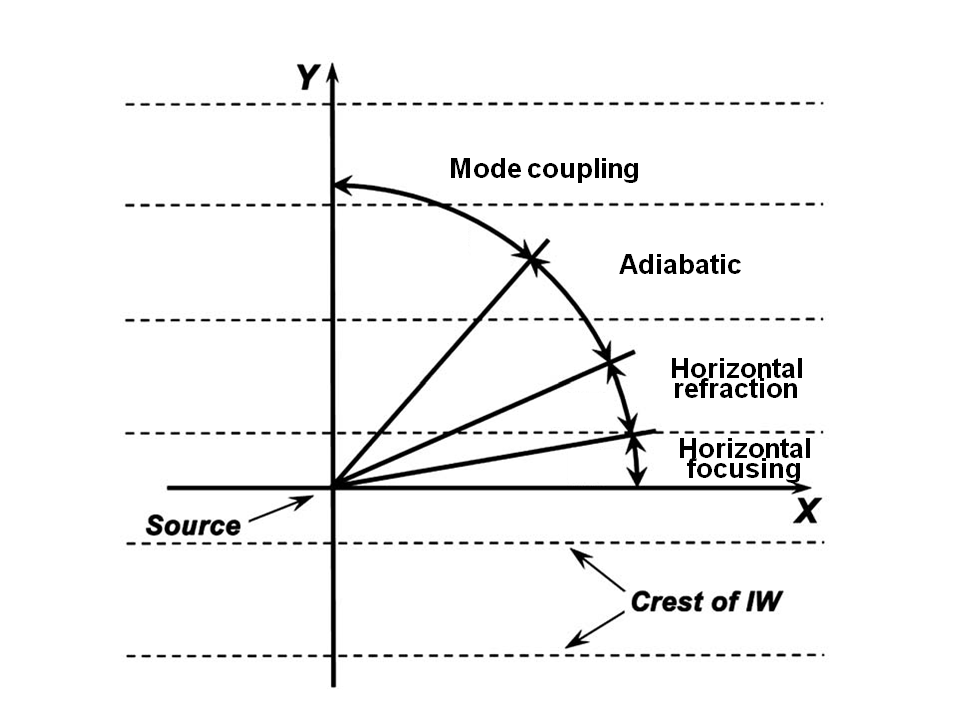
\includegraphics[width=0.75\textwidth]{angle3.png}\\
%  \caption{Schematic diagram showing the relationship between the IW crests and the acoustic propagation track.}
%  \label{fig:angle}
%\end{figure}
%
%%\section{Literature Search}
%\section{Thesis Outline}
%This thesis is divided in 6 chapters. In Chapter 2 we present the theory of acoustic wave propagation in waveguides in the presence of internal waves. We will also present the theory of vertical modes and horizontal rays in the context of the shallow water acoustic wave propagation in the inhomogeneous anisotropic shallow water waveguides. Chapter 3 is dedicated to the detailed description of the experimental observation during the Shallow Water 2006 (SW06) experiment.
%In Chapter 4,we presents the analysis and computer modeling results for those observations. Chapter 5 summarizes the original contributions of this work.
